\documentclass[11pt]{article}

    \usepackage[breakable]{tcolorbox}
    \usepackage{parskip} % Stop auto-indenting (to mimic markdown behaviour)
    
    \usepackage{iftex}
    \ifPDFTeX
    	\usepackage[T1]{fontenc}
    	\usepackage{mathpazo}
    \else
    	\usepackage{fontspec}
    \fi

    % Basic figure setup, for now with no caption control since it's done
    % automatically by Pandoc (which extracts ![](path) syntax from Markdown).
    \usepackage{graphicx}
    % Maintain compatibility with old templates. Remove in nbconvert 6.0
    \let\Oldincludegraphics\includegraphics
    % Ensure that by default, figures have no caption (until we provide a
    % proper Figure object with a Caption API and a way to capture that
    % in the conversion process - todo).
    \usepackage{caption}
    % \DeclareCaptionFormat{nocaption}{}
    % \captionsetup{format=nocaption,aboveskip=0pt,belowskip=0pt}

    \usepackage[Export]{adjustbox} % Used to constrain images to a maximum size
    \adjustboxset{max size={0.9\linewidth}{0.9\paperheight}}
    \usepackage{float}
    \floatplacement{figure}{H} % forces figures to be placed at the correct location
    \usepackage{xcolor} % Allow colors to be defined
    \usepackage{enumerate} % Needed for markdown enumerations to work
    \usepackage{geometry} % Used to adjust the document margins
    \usepackage{amsmath} % Equations
    \usepackage{amssymb} % Equations
    \usepackage{textcomp} % defines textquotesingle
    % Hack from http://tex.stackexchange.com/a/47451/13684:
    \AtBeginDocument{%
        \def\PYZsq{\textquotesingle}% Upright quotes in Pygmentized code
    }
    \usepackage{upquote} % Upright quotes for verbatim code
    \usepackage{eurosym} % defines \euro
    \usepackage[mathletters]{ucs} % Extended unicode (utf-8) support
    \usepackage{fancyvrb} % verbatim replacement that allows latex
    \usepackage{grffile} % extends the file name processing of package graphics 
                         % to support a larger range
    \makeatletter % fix for grffile with XeLaTeX
    \def\Gread@@xetex#1{%
      \IfFileExists{"\Gin@base".bb}%
      {\Gread@eps{\Gin@base.bb}}%
      {\Gread@@xetex@aux#1}%
    }
    \makeatother

    % The hyperref package gives us a pdf with properly built
    % internal navigation ('pdf bookmarks' for the table of contents,
    % internal cross-reference links, web links for URLs, etc.)
    \usepackage{hyperref}
    % The default LaTeX title has an obnoxious amount of whitespace. By default,
    % titling removes some of it. It also provides customization options.
    \usepackage{titling}
    \usepackage{longtable} % longtable support required by pandoc >1.10
    \usepackage{booktabs}  % table support for pandoc > 1.12.2
    \usepackage[inline]{enumitem} % IRkernel/repr support (it uses the enumerate* environment)
    \usepackage[normalem]{ulem} % ulem is needed to support strikethroughs (\sout)
                                % normalem makes italics be italics, not underlines
    \usepackage{mathrsfs}
    

    
    % Colors for the hyperref package
    \definecolor{urlcolor}{rgb}{0,.145,.698}
    \definecolor{linkcolor}{rgb}{.71,0.21,0.01}
    \definecolor{citecolor}{rgb}{.12,.54,.11}

    % ANSI colors
    \definecolor{ansi-black}{HTML}{3E424D}
    \definecolor{ansi-black-intense}{HTML}{282C36}
    \definecolor{ansi-red}{HTML}{E75C58}
    \definecolor{ansi-red-intense}{HTML}{B22B31}
    \definecolor{ansi-green}{HTML}{00A250}
    \definecolor{ansi-green-intense}{HTML}{007427}
    \definecolor{ansi-yellow}{HTML}{DDB62B}
    \definecolor{ansi-yellow-intense}{HTML}{B27D12}
    \definecolor{ansi-blue}{HTML}{208FFB}
    \definecolor{ansi-blue-intense}{HTML}{0065CA}
    \definecolor{ansi-magenta}{HTML}{D160C4}
    \definecolor{ansi-magenta-intense}{HTML}{A03196}
    \definecolor{ansi-cyan}{HTML}{60C6C8}
    \definecolor{ansi-cyan-intense}{HTML}{258F8F}
    \definecolor{ansi-white}{HTML}{C5C1B4}
    \definecolor{ansi-white-intense}{HTML}{A1A6B2}
    \definecolor{ansi-default-inverse-fg}{HTML}{FFFFFF}
    \definecolor{ansi-default-inverse-bg}{HTML}{000000}

    % commands and environments needed by pandoc snippets
    % extracted from the output of `pandoc -s`
    \providecommand{\tightlist}{%
      \setlength{\itemsep}{0pt}\setlength{\parskip}{0pt}}
    \DefineVerbatimEnvironment{Highlighting}{Verbatim}{commandchars=\\\{\}}
    % Add ',fontsize=\small' for more characters per line
    \newenvironment{Shaded}{}{}
    \newcommand{\KeywordTok}[1]{\textcolor[rgb]{0.00,0.44,0.13}{\textbf{{#1}}}}
    \newcommand{\DataTypeTok}[1]{\textcolor[rgb]{0.56,0.13,0.00}{{#1}}}
    \newcommand{\DecValTok}[1]{\textcolor[rgb]{0.25,0.63,0.44}{{#1}}}
    \newcommand{\BaseNTok}[1]{\textcolor[rgb]{0.25,0.63,0.44}{{#1}}}
    \newcommand{\FloatTok}[1]{\textcolor[rgb]{0.25,0.63,0.44}{{#1}}}
    \newcommand{\CharTok}[1]{\textcolor[rgb]{0.25,0.44,0.63}{{#1}}}
    \newcommand{\StringTok}[1]{\textcolor[rgb]{0.25,0.44,0.63}{{#1}}}
    \newcommand{\CommentTok}[1]{\textcolor[rgb]{0.38,0.63,0.69}{\textit{{#1}}}}
    \newcommand{\OtherTok}[1]{\textcolor[rgb]{0.00,0.44,0.13}{{#1}}}
    \newcommand{\AlertTok}[1]{\textcolor[rgb]{1.00,0.00,0.00}{\textbf{{#1}}}}
    \newcommand{\FunctionTok}[1]{\textcolor[rgb]{0.02,0.16,0.49}{{#1}}}
    \newcommand{\RegionMarkerTok}[1]{{#1}}
    \newcommand{\ErrorTok}[1]{\textcolor[rgb]{1.00,0.00,0.00}{\textbf{{#1}}}}
    \newcommand{\NormalTok}[1]{{#1}}
    
    % Additional commands for more recent versions of Pandoc
    \newcommand{\ConstantTok}[1]{\textcolor[rgb]{0.53,0.00,0.00}{{#1}}}
    \newcommand{\SpecialCharTok}[1]{\textcolor[rgb]{0.25,0.44,0.63}{{#1}}}
    \newcommand{\VerbatimStringTok}[1]{\textcolor[rgb]{0.25,0.44,0.63}{{#1}}}
    \newcommand{\SpecialStringTok}[1]{\textcolor[rgb]{0.73,0.40,0.53}{{#1}}}
    \newcommand{\ImportTok}[1]{{#1}}
    \newcommand{\DocumentationTok}[1]{\textcolor[rgb]{0.73,0.13,0.13}{\textit{{#1}}}}
    \newcommand{\AnnotationTok}[1]{\textcolor[rgb]{0.38,0.63,0.69}{\textbf{\textit{{#1}}}}}
    \newcommand{\CommentVarTok}[1]{\textcolor[rgb]{0.38,0.63,0.69}{\textbf{\textit{{#1}}}}}
    \newcommand{\VariableTok}[1]{\textcolor[rgb]{0.10,0.09,0.49}{{#1}}}
    \newcommand{\ControlFlowTok}[1]{\textcolor[rgb]{0.00,0.44,0.13}{\textbf{{#1}}}}
    \newcommand{\OperatorTok}[1]{\textcolor[rgb]{0.40,0.40,0.40}{{#1}}}
    \newcommand{\BuiltInTok}[1]{{#1}}
    \newcommand{\ExtensionTok}[1]{{#1}}
    \newcommand{\PreprocessorTok}[1]{\textcolor[rgb]{0.74,0.48,0.00}{{#1}}}
    \newcommand{\AttributeTok}[1]{\textcolor[rgb]{0.49,0.56,0.16}{{#1}}}
    \newcommand{\InformationTok}[1]{\textcolor[rgb]{0.38,0.63,0.69}{\textbf{\textit{{#1}}}}}
    \newcommand{\WarningTok}[1]{\textcolor[rgb]{0.38,0.63,0.69}{\textbf{\textit{{#1}}}}}
    
    
    % Define a nice break command that doesn't care if a line doesn't already
    % exist.
    \def\br{\hspace*{\fill} \\* }
    % Math Jax compatibility definitions
    \def\gt{>}
    \def\lt{<}
    \let\Oldtex\TeX
    \let\Oldlatex\LaTeX
    \renewcommand{\TeX}{\textrm{\Oldtex}}
    \renewcommand{\LaTeX}{\textrm{\Oldlatex}}
    % Document parameters
    % Document title
    
\title{I tassi di riproduzione nelle epidemie}

    
    
\author{Max Pierini$^*$}
\date{%
    $^*$\href{mailto:info@maxpierini.it}{info@maxpierini.it}\\%
    \href{https://t.me/notiziae}{NOTIZI\AE}\\%
    \href{https://maxpierini.it/ncov}{nCoV website}\\[2ex]%
    \today
}

    
% Pygments definitions
\makeatletter
\def\PY@reset{\let\PY@it=\relax \let\PY@bf=\relax%
    \let\PY@ul=\relax \let\PY@tc=\relax%
    \let\PY@bc=\relax \let\PY@ff=\relax}
\def\PY@tok#1{\csname PY@tok@#1\endcsname}
\def\PY@toks#1+{\ifx\relax#1\empty\else%
    \PY@tok{#1}\expandafter\PY@toks\fi}
\def\PY@do#1{\PY@bc{\PY@tc{\PY@ul{%
    \PY@it{\PY@bf{\PY@ff{#1}}}}}}}
\def\PY#1#2{\PY@reset\PY@toks#1+\relax+\PY@do{#2}}

\expandafter\def\csname PY@tok@w\endcsname{\def\PY@tc##1{\textcolor[rgb]{0.73,0.73,0.73}{##1}}}
\expandafter\def\csname PY@tok@c\endcsname{\let\PY@it=\textit\def\PY@tc##1{\textcolor[rgb]{0.25,0.50,0.50}{##1}}}
\expandafter\def\csname PY@tok@cp\endcsname{\def\PY@tc##1{\textcolor[rgb]{0.74,0.48,0.00}{##1}}}
\expandafter\def\csname PY@tok@k\endcsname{\let\PY@bf=\textbf\def\PY@tc##1{\textcolor[rgb]{0.00,0.50,0.00}{##1}}}
\expandafter\def\csname PY@tok@kp\endcsname{\def\PY@tc##1{\textcolor[rgb]{0.00,0.50,0.00}{##1}}}
\expandafter\def\csname PY@tok@kt\endcsname{\def\PY@tc##1{\textcolor[rgb]{0.69,0.00,0.25}{##1}}}
\expandafter\def\csname PY@tok@o\endcsname{\def\PY@tc##1{\textcolor[rgb]{0.40,0.40,0.40}{##1}}}
\expandafter\def\csname PY@tok@ow\endcsname{\let\PY@bf=\textbf\def\PY@tc##1{\textcolor[rgb]{0.67,0.13,1.00}{##1}}}
\expandafter\def\csname PY@tok@nb\endcsname{\def\PY@tc##1{\textcolor[rgb]{0.00,0.50,0.00}{##1}}}
\expandafter\def\csname PY@tok@nf\endcsname{\def\PY@tc##1{\textcolor[rgb]{0.00,0.00,1.00}{##1}}}
\expandafter\def\csname PY@tok@nc\endcsname{\let\PY@bf=\textbf\def\PY@tc##1{\textcolor[rgb]{0.00,0.00,1.00}{##1}}}
\expandafter\def\csname PY@tok@nn\endcsname{\let\PY@bf=\textbf\def\PY@tc##1{\textcolor[rgb]{0.00,0.00,1.00}{##1}}}
\expandafter\def\csname PY@tok@ne\endcsname{\let\PY@bf=\textbf\def\PY@tc##1{\textcolor[rgb]{0.82,0.25,0.23}{##1}}}
\expandafter\def\csname PY@tok@nv\endcsname{\def\PY@tc##1{\textcolor[rgb]{0.10,0.09,0.49}{##1}}}
\expandafter\def\csname PY@tok@no\endcsname{\def\PY@tc##1{\textcolor[rgb]{0.53,0.00,0.00}{##1}}}
\expandafter\def\csname PY@tok@nl\endcsname{\def\PY@tc##1{\textcolor[rgb]{0.63,0.63,0.00}{##1}}}
\expandafter\def\csname PY@tok@ni\endcsname{\let\PY@bf=\textbf\def\PY@tc##1{\textcolor[rgb]{0.60,0.60,0.60}{##1}}}
\expandafter\def\csname PY@tok@na\endcsname{\def\PY@tc##1{\textcolor[rgb]{0.49,0.56,0.16}{##1}}}
\expandafter\def\csname PY@tok@nt\endcsname{\let\PY@bf=\textbf\def\PY@tc##1{\textcolor[rgb]{0.00,0.50,0.00}{##1}}}
\expandafter\def\csname PY@tok@nd\endcsname{\def\PY@tc##1{\textcolor[rgb]{0.67,0.13,1.00}{##1}}}
\expandafter\def\csname PY@tok@s\endcsname{\def\PY@tc##1{\textcolor[rgb]{0.73,0.13,0.13}{##1}}}
\expandafter\def\csname PY@tok@sd\endcsname{\let\PY@it=\textit\def\PY@tc##1{\textcolor[rgb]{0.73,0.13,0.13}{##1}}}
\expandafter\def\csname PY@tok@si\endcsname{\let\PY@bf=\textbf\def\PY@tc##1{\textcolor[rgb]{0.73,0.40,0.53}{##1}}}
\expandafter\def\csname PY@tok@se\endcsname{\let\PY@bf=\textbf\def\PY@tc##1{\textcolor[rgb]{0.73,0.40,0.13}{##1}}}
\expandafter\def\csname PY@tok@sr\endcsname{\def\PY@tc##1{\textcolor[rgb]{0.73,0.40,0.53}{##1}}}
\expandafter\def\csname PY@tok@ss\endcsname{\def\PY@tc##1{\textcolor[rgb]{0.10,0.09,0.49}{##1}}}
\expandafter\def\csname PY@tok@sx\endcsname{\def\PY@tc##1{\textcolor[rgb]{0.00,0.50,0.00}{##1}}}
\expandafter\def\csname PY@tok@m\endcsname{\def\PY@tc##1{\textcolor[rgb]{0.40,0.40,0.40}{##1}}}
\expandafter\def\csname PY@tok@gh\endcsname{\let\PY@bf=\textbf\def\PY@tc##1{\textcolor[rgb]{0.00,0.00,0.50}{##1}}}
\expandafter\def\csname PY@tok@gu\endcsname{\let\PY@bf=\textbf\def\PY@tc##1{\textcolor[rgb]{0.50,0.00,0.50}{##1}}}
\expandafter\def\csname PY@tok@gd\endcsname{\def\PY@tc##1{\textcolor[rgb]{0.63,0.00,0.00}{##1}}}
\expandafter\def\csname PY@tok@gi\endcsname{\def\PY@tc##1{\textcolor[rgb]{0.00,0.63,0.00}{##1}}}
\expandafter\def\csname PY@tok@gr\endcsname{\def\PY@tc##1{\textcolor[rgb]{1.00,0.00,0.00}{##1}}}
\expandafter\def\csname PY@tok@ge\endcsname{\let\PY@it=\textit}
\expandafter\def\csname PY@tok@gs\endcsname{\let\PY@bf=\textbf}
\expandafter\def\csname PY@tok@gp\endcsname{\let\PY@bf=\textbf\def\PY@tc##1{\textcolor[rgb]{0.00,0.00,0.50}{##1}}}
\expandafter\def\csname PY@tok@go\endcsname{\def\PY@tc##1{\textcolor[rgb]{0.53,0.53,0.53}{##1}}}
\expandafter\def\csname PY@tok@gt\endcsname{\def\PY@tc##1{\textcolor[rgb]{0.00,0.27,0.87}{##1}}}
\expandafter\def\csname PY@tok@err\endcsname{\def\PY@bc##1{\setlength{\fboxsep}{0pt}\fcolorbox[rgb]{1.00,0.00,0.00}{1,1,1}{\strut ##1}}}
\expandafter\def\csname PY@tok@kc\endcsname{\let\PY@bf=\textbf\def\PY@tc##1{\textcolor[rgb]{0.00,0.50,0.00}{##1}}}
\expandafter\def\csname PY@tok@kd\endcsname{\let\PY@bf=\textbf\def\PY@tc##1{\textcolor[rgb]{0.00,0.50,0.00}{##1}}}
\expandafter\def\csname PY@tok@kn\endcsname{\let\PY@bf=\textbf\def\PY@tc##1{\textcolor[rgb]{0.00,0.50,0.00}{##1}}}
\expandafter\def\csname PY@tok@kr\endcsname{\let\PY@bf=\textbf\def\PY@tc##1{\textcolor[rgb]{0.00,0.50,0.00}{##1}}}
\expandafter\def\csname PY@tok@bp\endcsname{\def\PY@tc##1{\textcolor[rgb]{0.00,0.50,0.00}{##1}}}
\expandafter\def\csname PY@tok@fm\endcsname{\def\PY@tc##1{\textcolor[rgb]{0.00,0.00,1.00}{##1}}}
\expandafter\def\csname PY@tok@vc\endcsname{\def\PY@tc##1{\textcolor[rgb]{0.10,0.09,0.49}{##1}}}
\expandafter\def\csname PY@tok@vg\endcsname{\def\PY@tc##1{\textcolor[rgb]{0.10,0.09,0.49}{##1}}}
\expandafter\def\csname PY@tok@vi\endcsname{\def\PY@tc##1{\textcolor[rgb]{0.10,0.09,0.49}{##1}}}
\expandafter\def\csname PY@tok@vm\endcsname{\def\PY@tc##1{\textcolor[rgb]{0.10,0.09,0.49}{##1}}}
\expandafter\def\csname PY@tok@sa\endcsname{\def\PY@tc##1{\textcolor[rgb]{0.73,0.13,0.13}{##1}}}
\expandafter\def\csname PY@tok@sb\endcsname{\def\PY@tc##1{\textcolor[rgb]{0.73,0.13,0.13}{##1}}}
\expandafter\def\csname PY@tok@sc\endcsname{\def\PY@tc##1{\textcolor[rgb]{0.73,0.13,0.13}{##1}}}
\expandafter\def\csname PY@tok@dl\endcsname{\def\PY@tc##1{\textcolor[rgb]{0.73,0.13,0.13}{##1}}}
\expandafter\def\csname PY@tok@s2\endcsname{\def\PY@tc##1{\textcolor[rgb]{0.73,0.13,0.13}{##1}}}
\expandafter\def\csname PY@tok@sh\endcsname{\def\PY@tc##1{\textcolor[rgb]{0.73,0.13,0.13}{##1}}}
\expandafter\def\csname PY@tok@s1\endcsname{\def\PY@tc##1{\textcolor[rgb]{0.73,0.13,0.13}{##1}}}
\expandafter\def\csname PY@tok@mb\endcsname{\def\PY@tc##1{\textcolor[rgb]{0.40,0.40,0.40}{##1}}}
\expandafter\def\csname PY@tok@mf\endcsname{\def\PY@tc##1{\textcolor[rgb]{0.40,0.40,0.40}{##1}}}
\expandafter\def\csname PY@tok@mh\endcsname{\def\PY@tc##1{\textcolor[rgb]{0.40,0.40,0.40}{##1}}}
\expandafter\def\csname PY@tok@mi\endcsname{\def\PY@tc##1{\textcolor[rgb]{0.40,0.40,0.40}{##1}}}
\expandafter\def\csname PY@tok@il\endcsname{\def\PY@tc##1{\textcolor[rgb]{0.40,0.40,0.40}{##1}}}
\expandafter\def\csname PY@tok@mo\endcsname{\def\PY@tc##1{\textcolor[rgb]{0.40,0.40,0.40}{##1}}}
\expandafter\def\csname PY@tok@ch\endcsname{\let\PY@it=\textit\def\PY@tc##1{\textcolor[rgb]{0.25,0.50,0.50}{##1}}}
\expandafter\def\csname PY@tok@cm\endcsname{\let\PY@it=\textit\def\PY@tc##1{\textcolor[rgb]{0.25,0.50,0.50}{##1}}}
\expandafter\def\csname PY@tok@cpf\endcsname{\let\PY@it=\textit\def\PY@tc##1{\textcolor[rgb]{0.25,0.50,0.50}{##1}}}
\expandafter\def\csname PY@tok@c1\endcsname{\let\PY@it=\textit\def\PY@tc##1{\textcolor[rgb]{0.25,0.50,0.50}{##1}}}
\expandafter\def\csname PY@tok@cs\endcsname{\let\PY@it=\textit\def\PY@tc##1{\textcolor[rgb]{0.25,0.50,0.50}{##1}}}

\def\PYZbs{\char`\\}
\def\PYZus{\char`\_}
\def\PYZob{\char`\{}
\def\PYZcb{\char`\}}
\def\PYZca{\char`\^}
\def\PYZam{\char`\&}
\def\PYZlt{\char`\<}
\def\PYZgt{\char`\>}
\def\PYZsh{\char`\#}
\def\PYZpc{\char`\%}
\def\PYZdl{\char`\$}
\def\PYZhy{\char`\-}
\def\PYZsq{\char`\'}
\def\PYZdq{\char`\"}
\def\PYZti{\char`\~}
% for compatibility with earlier versions
\def\PYZat{@}
\def\PYZlb{[}
\def\PYZrb{]}
\makeatother


    % For linebreaks inside Verbatim environment from package fancyvrb. 
    \makeatletter
        \newbox\Wrappedcontinuationbox 
        \newbox\Wrappedvisiblespacebox 
        \newcommand*\Wrappedvisiblespace {\textcolor{red}{\textvisiblespace}} 
        \newcommand*\Wrappedcontinuationsymbol {\textcolor{red}{\llap{\tiny$\m@th\hookrightarrow$}}} 
        \newcommand*\Wrappedcontinuationindent {3ex } 
        \newcommand*\Wrappedafterbreak {\kern\Wrappedcontinuationindent\copy\Wrappedcontinuationbox} 
        % Take advantage of the already applied Pygments mark-up to insert 
        % potential linebreaks for TeX processing. 
        %        {, <, #, %, $, ' and ": go to next line. 
        %        _, }, ^, &, >, - and ~: stay at end of broken line. 
        % Use of \textquotesingle for straight quote. 
        \newcommand*\Wrappedbreaksatspecials {% 
            \def\PYGZus{\discretionary{\char`\_}{\Wrappedafterbreak}{\char`\_}}% 
            \def\PYGZob{\discretionary{}{\Wrappedafterbreak\char`\{}{\char`\{}}% 
            \def\PYGZcb{\discretionary{\char`\}}{\Wrappedafterbreak}{\char`\}}}% 
            \def\PYGZca{\discretionary{\char`\^}{\Wrappedafterbreak}{\char`\^}}% 
            \def\PYGZam{\discretionary{\char`\&}{\Wrappedafterbreak}{\char`\&}}% 
            \def\PYGZlt{\discretionary{}{\Wrappedafterbreak\char`\<}{\char`\<}}% 
            \def\PYGZgt{\discretionary{\char`\>}{\Wrappedafterbreak}{\char`\>}}% 
            \def\PYGZsh{\discretionary{}{\Wrappedafterbreak\char`\#}{\char`\#}}% 
            \def\PYGZpc{\discretionary{}{\Wrappedafterbreak\char`\%}{\char`\%}}% 
            \def\PYGZdl{\discretionary{}{\Wrappedafterbreak\char`\$}{\char`\$}}% 
            \def\PYGZhy{\discretionary{\char`\-}{\Wrappedafterbreak}{\char`\-}}% 
            \def\PYGZsq{\discretionary{}{\Wrappedafterbreak\textquotesingle}{\textquotesingle}}% 
            \def\PYGZdq{\discretionary{}{\Wrappedafterbreak\char`\"}{\char`\"}}% 
            \def\PYGZti{\discretionary{\char`\~}{\Wrappedafterbreak}{\char`\~}}% 
        } 
        % Some characters . , ; ? ! / are not pygmentized. 
        % This macro makes them "active" and they will insert potential linebreaks 
        \newcommand*\Wrappedbreaksatpunct {% 
            \lccode`\~`\.\lowercase{\def~}{\discretionary{\hbox{\char`\.}}{\Wrappedafterbreak}{\hbox{\char`\.}}}% 
            \lccode`\~`\,\lowercase{\def~}{\discretionary{\hbox{\char`\,}}{\Wrappedafterbreak}{\hbox{\char`\,}}}% 
            \lccode`\~`\;\lowercase{\def~}{\discretionary{\hbox{\char`\;}}{\Wrappedafterbreak}{\hbox{\char`\;}}}% 
            \lccode`\~`\:\lowercase{\def~}{\discretionary{\hbox{\char`\:}}{\Wrappedafterbreak}{\hbox{\char`\:}}}% 
            \lccode`\~`\?\lowercase{\def~}{\discretionary{\hbox{\char`\?}}{\Wrappedafterbreak}{\hbox{\char`\?}}}% 
            \lccode`\~`\!\lowercase{\def~}{\discretionary{\hbox{\char`\!}}{\Wrappedafterbreak}{\hbox{\char`\!}}}% 
            \lccode`\~`\/\lowercase{\def~}{\discretionary{\hbox{\char`\/}}{\Wrappedafterbreak}{\hbox{\char`\/}}}% 
            \catcode`\.\active
            \catcode`\,\active 
            \catcode`\;\active
            \catcode`\:\active
            \catcode`\?\active
            \catcode`\!\active
            \catcode`\/\active 
            \lccode`\~`\~ 	
        }
    \makeatother

    \let\OriginalVerbatim=\Verbatim
    \makeatletter
    \renewcommand{\Verbatim}[1][1]{%
        %\parskip\z@skip
        \sbox\Wrappedcontinuationbox {\Wrappedcontinuationsymbol}%
        \sbox\Wrappedvisiblespacebox {\FV@SetupFont\Wrappedvisiblespace}%
        \def\FancyVerbFormatLine ##1{\hsize\linewidth
            \vtop{\raggedright\hyphenpenalty\z@\exhyphenpenalty\z@
                \doublehyphendemerits\z@\finalhyphendemerits\z@
                \strut ##1\strut}%
        }%
        % If the linebreak is at a space, the latter will be displayed as visible
        % space at end of first line, and a continuation symbol starts next line.
        % Stretch/shrink are however usually zero for typewriter font.
        \def\FV@Space {%
            \nobreak\hskip\z@ plus\fontdimen3\font minus\fontdimen4\font
            \discretionary{\copy\Wrappedvisiblespacebox}{\Wrappedafterbreak}
            {\kern\fontdimen2\font}%
        }%
        
        % Allow breaks at special characters using \PYG... macros.
        \Wrappedbreaksatspecials
        % Breaks at punctuation characters . , ; ? ! and / need catcode=\active 	
        \OriginalVerbatim[#1,codes*=\Wrappedbreaksatpunct]%
    }
    \makeatother

    % Exact colors from NB
    \definecolor{incolor}{HTML}{303F9F}
    \definecolor{outcolor}{HTML}{D84315}
    \definecolor{cellborder}{HTML}{CFCFCF}
    \definecolor{cellbackground}{HTML}{F7F7F7}
    
    % prompt
    \makeatletter
    \newcommand{\boxspacing}{\kern\kvtcb@left@rule\kern\kvtcb@boxsep}
    \makeatother
    \newcommand{\prompt}[4]{
        \ttfamily\llap{{\color{#2}[#3]:\hspace{3pt}#4}}\vspace{-\baselineskip}
    }
    

    
    % Prevent overflowing lines due to hard-to-break entities
    \sloppy 
    % Setup hyperref package
    \hypersetup{
      breaklinks=true,  % so long urls are correctly broken across lines
      colorlinks=true,
      urlcolor=urlcolor,
      linkcolor=linkcolor,
      citecolor=citecolor,
      }
    % Slightly bigger margins than the latex defaults
    
    \geometry{verbose,tmargin=1in,bmargin=1in,lmargin=1in,rmargin=1in}
    
    

\begin{document}
    
    \maketitle
    
    

    
    \hypertarget{i-tassi-di-riproduzione-re_0-e-re_t}{%
\section{\texorpdfstring{I tassi di riproduzione: \(\Re_0\) e
\(\Re_t\)}{I tassi di riproduzione: \textbackslash Re\_0 e \textbackslash Re\_t}}\label{i-tassi-di-riproduzione-re_0-e-re_t}}

    \hypertarget{il-modello-sird}{%
\subsection{\texorpdfstring{Il modello
\textbf{SIRD}}{Il modello SIRD}}\label{il-modello-sird}}

    I processi di diffusione delle epidemie sono notevolmente complessi e
dipendono da numerosi fattori. È tuttavia possibile, grazie all'utilizzo
di specifici modelli matematici, stimare l'andamento di un'epidemia al
fine di valutarne l'evoluzione naturale e/o l'efficacia delle
contromisure di contenimento (distanziamento sociale, lockdown, ecc).

I modelli più spesso utilizzati sono di tipo compartimentale
\cite{fassina2013modelli}: la popolazione viene suddivisa in
\emph{compartimenti} e il passaggio dei soggetti da un compartimento
all'altro è definito da regole probabilistiche notevolmente
semplificate.

Uno dei modelli compartimentali più usati per le malattie infettive è il
\textbf{SIRD} \cite{ep_repository_2020}. La popolazione è suddivisa in:

\begin{itemize}
\item
  \textbf{S}: Suscettibili. Tutti coloro che non hanno contratto la
  malattia e potrebbero essere contagiati.
\item
  \textbf{I}: Infetti. Coloro che hanno contratto la malattia, non sono
  guariti e potrebbero contagiare uno o più Suscettibili.
\item
  \textbf{R}: Guariti (dall'inglese \emph{Recovered}). I soggetti che
  hanno contratto la malattia e ne sono guariti.
\item
  \textbf{D}: Deceduti. Tutti coloro che sono deceduti a causa della
  malattia specifica contratta in precedenza.
\end{itemize}

Le \emph{regole di transizione} descrivono la possibilità di passaggio
dei soggetti da un compartimento all'altro \(fig. \ref{fig:sird}\) (in alcuni
modelli più semplici, \(\mathbf{R}\) e \(\mathbf{D}\) sono `uniti' in un
unico comparto \(\mathbf{R}\), Rimossi, e il passaggio da Infetti a
Rimossi è regolato dal tasso di rimozione, modello \textbf{\emph{SIR}}).

    \begin{figure}
\centering
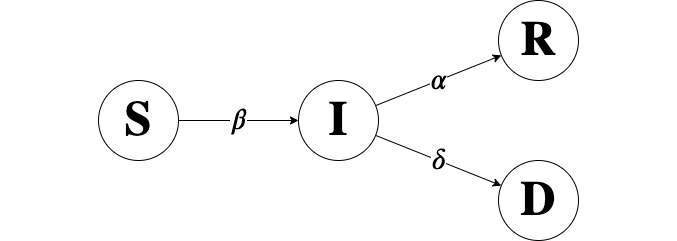
\includegraphics{images/sird.png}
\caption{Struttura del modello \textbf{SIRD}}
\label{fig:sird}
\end{figure}

    Il passaggio da Suscettibili \(\mathbf{S}\) a Infetti \(\mathbf{I}\) è
determinato dal parametro di transizione \(\beta\) (da cui dipende
direttamente il tasso di trasmissione della malattia). Un soggetto
infettato non può ``rientrare'' nei Suscettibili dato che, una volta
contratta la malattia, si suppone che svilupperà anticorpi e dunque non
potrà essere infettato nuovamente. Questa è un'assunzione fondamentale 
per il modello utilizzato. Nel caso invece di malattie infettive in cui un 
Infetto può perdere l'immunità (a causa ad esempio di mutazioni dell'agente infettante) 
o di malattie infettive endemiche (come l'influenza stagionale) esistono modelli specifici.

Il passaggio da Infetti \(\mathbf{I}\) a Guariti \(\mathbf{R}\) è
regolato dal tasso di guarigione \(\alpha\). Anche in questo caso, si
suppone che il soggetto non possa essere reinfettato e che un eventuale
decesso sia da attribuire a cause differenti dalla malattia in esame.

Il passaggio da Infetti \(\mathbf{I}\) a Deceduti \(\mathbf{D}\) è
invece descritto dal tasso di letalità \(\delta\).

    La quantità di soggetti presenti in ogni compartimento è, come si può
facilmente dedurre, variabile nel tempo \(t\).

Dunque parleremo di \(\mathbf{S}_t\), \(\mathbf{I}_t\), \(\mathbf{R}_t\)
e \(\mathbf{D}_t\) rispettivamente per Suscettibili, Infetti, Guariti e
Deceduti nel tempo \(t\).

In assenza di malattia, \(\mathbf{S}\) sarà pari all'intera popolazione,
che chiameremo \(\mathbf{N}\), mentre gli altri compartimenti saranno
vuoti.

Possiamo immaginare quindi l'inizio di una possibile epidemia generata
nel momento iniziale \(t=0\) da un singolo individuo Infetto
(\(\mathbf{I}_0 = 1\)) il quale può contagiare un certo numero di
Suscettibili.

Man mano che l'epidemia avanza (\(t_0 + \Delta t_1\) nella figura
\(\ref{fig:transird}\)), il numero di Infetti aumenterà e diminuirà il
numero dei Suscettibili.

Successivamente (\(t_0 + \Delta t_2\) nella figura
\(\ref{fig:transird}\)), alcuni soggetti inizieranno a guarire e per
altri il decorso risulterà fatale.

In questo caso ci riferiamo ad un \(\Delta\) temporale arbitrario.
Solitamente, nel corso di un'epidemia, i dati raccolti hanno cadenza
giornaliera. Dunque quando si parla di \(\Delta\) ci si riferisce
(laddove non altrimenti specificato) alla differenza giornaliera dei
dati.

    \begin{figure}
    \adjustimage{max size={0.9\linewidth}{0.9\paperheight}}{articolo-R0_files/articolo-R0_8_0.png}
    \caption{Transizioni nei compartimenti \textbf{SIRD} nel tempo.}
    \label{fig:transird}
    \end{figure}
    { \hspace*{\fill} \\}
    
    \hypertarget{il-tasso-netto-di-riproduzione-re_0}{%
\subsection{\texorpdfstring{Il tasso netto di riproduzione
\(\Re_0\)}{Il tasso netto di riproduzione \textbackslash Re\_0}}\label{il-tasso-netto-di-riproduzione-re_0}}

    Il numero medio di contagi generati dal primo Infetto in \(t=0\) è
chiamato appunto \emph{tasso netto di riproduzione} o \emph{numero di
riproduzione di base} \(\Re_0\) \cite{jones_2007}.

    Nella figura \(\ref{fig:r0ex}\) dunque, il tasso di riproduzione di base
sarà \(\Re_0 = 3\), ovvero: il primo individuo infetto ne può contagiare
in media 3, ciascuno di loro ne potrà contagiare altri 3, eccetera.

Quindi al tempo \(t=1\), gli Infetti saranno quattro,
\(\mathbf{I}_1 = 4\) e i Suscettibili saranno l'intera popolazione meno
i quattro individui Infetti ovvero
\(\mathbf{S}_1 = \mathbf{N} - \mathbf{I}_1 = \mathbf{N} - 4\).

Al tempo \(t=2\), gli Infetti saranno già tredici, \(\mathbf{I}_2 = 13\)
e i Suscettibili saranno l'intera popolazione meno i tredici soggetti
Infetti ovvero
\(\mathbf{S}_2 = \mathbf{N} - \mathbf{I}_2 = \mathbf{N} - 13\)

Più elevato è il numero di riproduzione di base \(\Re_0\) più
velocemente si propagherà un'epidemia.

Per ciascuna malattia infettiva, viene calcolato (e ricalcolato) un
tasso di riproduzione di base medio che diventa dunque un indice del
grado di contagiosità della malattia, utile per comparare tra di loro
differenti patologie ed eventuali modifiche del grado di contagiosità di
una malattia in tempi e/o luoghi differenti.

Concludendo la linea temporale, al termine dell'epidemia nel tempo
\(t_{\omega}\), il compartimento degli Infetti sarà nuovamente vuoto ma
avremo una certa quantità di Guariti e Deceduti e la popolazione
Suscettibile (in caso di una nuova epidemia della stessa malattia) sarà
dunque ridotta a
\(\mathbf{S}_{\omega} = \mathbf{N} - (\mathbf{R}_{\omega} + \mathbf{D}_{\omega})\).

    \begin{figure}
\centering
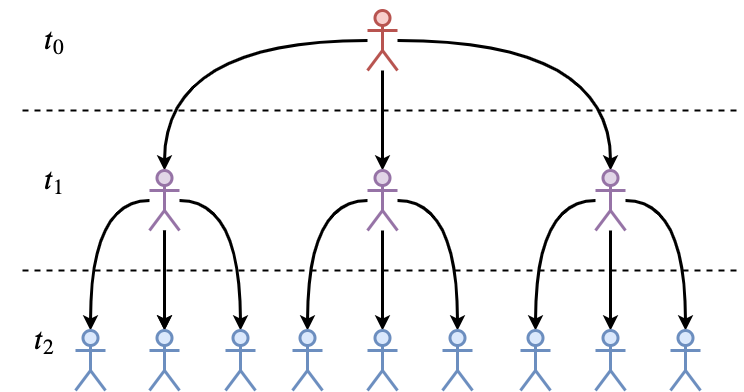
\includegraphics{images/r0.png}
\caption{Esempio di numero di riproduzione di base \(\Re_0 = 3\).}
\label{fig:r0ex}
\end{figure}

    Fin qui abbiamo però considerato il tasso di riproduzione come una
quantità costante.

È però intuibile che durante un'epidemia il passaggio dei soggetti da un
compartimento all'altro non sia costante ma si modifichi nel tempo. Ad
esempio:

\begin{itemize}
\item
  le contromisure di distanziamento sociale e i lockdown possono (e sono
  volti propriamente a) diminuire il più possibile il tasso di
  trasmissione \(\beta\)
\item
  nuove cure, farmaci o vaccini possono influire positivamente sia sul
  tasso di guarigione \(\alpha\) che sul tasso di letalità \(\delta\).
\end{itemize}

Queste variazioni nel tempo dei tassi di transizione possono a loro
volta influire sulla quantità di soggetti mediamente infettati e dunque
su \(\Re_0\) \cite{department_of_health} \cite{ceps_pubblication}
\cite{kissler_tedijanto_lipsitch_grad_2020}.

Dal punto di vista matematico infatti, \(\Re_0\) dipende dai tre tassi
di transizione (dove \(\Delta\) si riferisce in questo caso alle
variazioni giornaliere dei compartimenti):

\[ \Re_0 = \frac{ \Delta\mathbf{I} + (\Delta\mathbf{R} + \Delta\mathbf{D})}{ \Delta\mathbf{R} + \Delta\mathbf{D} } = \frac{ \beta \; \mathbf{I}_0 \; \mathbf{S}_0 }{ \alpha \; \mathbf{I}_0 + \delta \; \mathbf{I}_0} \]

ma dato che, come abbiamo visto precedentemente, all'istante iniziale
\(t=0\) il compartimento degli Infetti contiene un solo soggetto
\(\mathbf{I}_0 = 1\)

\[ \Re_0 = \frac{ \beta \; \mathbf{S}_0 }{ \alpha + \delta } \]

Visto in quest'ottica, \(\Re_0\) perde il significato di numero di
riproduzione di base ma diventa un utile indice di diffusione
dell'epidemia: non più quindi la quantità di contagi generati da
un'individuo infetto al tempo iniziale \(t_0\) bensì il rapporto
variabile nel tempo tra il tasso di trasmissione e i tassi di rimozione,
ovvero tra la variazione giornaliera di nuovi Infetti e nuovi Guariti o
Deceduti.

Se il numero di riproduzione di base nel tempo resta maggiore di 1
(\(\Re_0 > 1\)) significa che il numero di nuovi Infetti è maggiore del
numero giornaliero di Guariti o Deceduti e dunque l'epidemia continuerà
ad alimentarsi. Quando invece scende al di sotto dell'unità
(\(\Re_0 < 1\)) l'epidemia è sotto controllo e tenderà ad estinguersi
(più o meno velocemente) perché il numero giornaliero di nuovi Guariti o
Deceduti è maggiore del numero di nuovi Infetti.

    \hypertarget{il-tasso-di-riproduzione-effettivo-re_t}{%
\subsection{\texorpdfstring{Il tasso di riproduzione effettivo
\(\Re_t\)}{Il tasso di riproduzione effettivo \textbackslash Re\_t}}\label{il-tasso-di-riproduzione-effettivo-re_t}}

    Analizzando popolazioni di ridotte dimensioni, è possibile anche
affidarsi al calcolo del \emph{tasso di riproduzione effettivo}
\(\Re_t\) per una valutazione a medio/lungo termine di un'epidemia
\cite{k-sys} \cite{bettencourt_ribeiro_2008}.

\[ \Re_t = \Re_0 \frac{\mathbf{S}_t}{\mathbf{S}_0} \]

L'utilità di \(\Re_t\) è che può variare nel tempo anche in caso di un
\(\Re_0\) costante, ovvero anche nel caso in cui le contromisure di
contenimento non siano efficaci o non siano state applicate e/o nessuna
nuova cura migliori il tasso di guarigione o influisca sul tasso di
mortalità. È anche dunque un parametro utile per valutare il corso
naturale di un'epidemia in assenza di interventi contenitivi o medici.

    \hypertarget{calcoli-ed-esempi-italia}{%
\subsection{Calcoli ed esempi: Italia}\label{calcoli-ed-esempi-italia}}

    Mostreremo di seguito alcuni semplici esempi di calcolo di \(\Re_0\) ed
\(\Re_t\) basati sui dati italiani pubblicati dal Dipartimento di
Protezione Civile \cite{pcm_dpc_2020}.

    \hypertarget{re_0-statico}{%
\subsubsection{\texorpdfstring{\(\Re_0\)
``statico''}{\textbackslash Re\_0 ``statico''}}\label{re_0-statico}}

    La stima di \(\Re_0\) ``statico'' è notevolmente complessa e dipende da
numerosi fattori, tra cui i più importanti

\begin{itemize}
\item
  la scelta accurata del tempo iniziale \(t_0\)
\item
  le caratteristiche demografiche della popolazione esaminata
\item
  le vie e la dinamica di trasmissione del contagio
\item
  il tracciamento dei contatti
\item
  l'età e il sesso della popolazione considerata
\end{itemize}

tutti questi parametri possono influire sul numero di riproduzione di
base caratteristico della malattia in esame
\cite{delamater_street_leslie_yang_jacobsen_2019} \cite{report_2020}.

Per COVID-19, l'Organizzazione Mondiale della Sanità e numerosi altri
centri di ricerca nel mondo hanno pubblicato stime di \(\Re_0\) che sono
comprese tra \(1.4\) e \(5.7\) \cite{report_2020}. Per avere un termine
di paragone, ad esempio, la varicella ha un numero di riproduzione di
base di \(10\)-\(12\) e l'influenza stagionale di \(0.9\)-\(2.1\)
\cite{wikipedia_2020}. Dunque COVID-19 ha un \(\Re_0\) piuttosto
elevato.

    \hypertarget{re_0-dinamico}{%
\subsubsection{\texorpdfstring{\(\Re_0\)
``dinamico''}{\textbackslash Re\_0 ``dinamico''}}\label{re_0-dinamico}}

    \(\Re_0\) ``dinamico'' può essere calcolato con diversi metodi e diversi
modelli matematici. Utilizzando il modello \textbf{SIRD}, il calcolo più
semplice possibile si riduce al rapporto tra la variazione giornaliera
di nuovi Infetti e la variazione di nuovi Guariti e Deceduti
\cite{ep_repository_2020}:

\[ \Re_0 = \frac{ \Delta\mathbf{I} }{ \Delta\mathbf{R} + \Delta\mathbf{D} } + 1 \]

vediamo un esempio di applicazione di questa formula semplificata sui
casi di COVID-19 in Italia (fig. \(\ref{fig:r0it}\)), ``smussando'' il più possibile la
variabilità dei dati giornalieri dovuta a errori, correzioni, numero di
tamponi effettuati e comunicazione dei risultati, eccetera.

    \begin{figure}
    \adjustimage{max size={0.9\linewidth}{0.9\paperheight}}{articolo-R0_files/articolo-R0_26_0.png}
    \caption{\(\Re_0\) "dinamico" di COVID-19 in Italia.}
    \label{fig:r0it}
    \end{figure}
    { \hspace*{\fill} \\}
    
    Ricordiamo che, come detto in precedenza, nel caso di calcolo di
\(\Re_0\) dinamico il suo significato non è più quello del numero di
riproduzione di base, ovvero del numero di soggetti contagiati
mediamente da un infetto, ma solo di un valore soglia: quando \(\Re_0\)
è minore di \(1\) l'epidemia è sotto controllo.

Notiamo che dal 21 Aprile \(\Re_0 < 1\) dunque ci sono buone probabilità
che l'epidemia di COVID-19 sia in via di estinzione. Ma vediamo anche
però che è ``intorno a 1'' il che indica che le misure di contenimento
non possono essere abbandonate troppo velocemente: l'abbattimento di
\(\Re_0\) in questo caso dipende proprio dall'effetto positivo delle
contromisure adottate.\\
\\

    \begin{Verbatim}[commandchars=\\\{\}]
                           R0
data
2020-04-17 17:00:00  1.281164
2020-04-18 17:00:00  1.200606
2020-04-19 17:00:00  1.114617
2020-04-20 17:00:00  1.020266
2020-04-21 17:00:00  0.955652
2020-04-22 17:00:00  0.897395
2020-04-23 17:00:00  0.877171
2020-04-24 17:00:00  0.874121
2020-04-25 17:00:00  0.886059
2020-04-26 17:00:00  0.896871
    \end{Verbatim}

    \hypertarget{re_t}{%
\subsubsection{\texorpdfstring{\(\Re_t\)}{\textbackslash Re\_t}}\label{re_t}}

    Come si accennava, per il calcolo di \(\Re_t\) la popolazione non deve
essere eccessivamente ampia. L'intera popolazione italiana è troppo
numerosa per una stima efficace di \(\Re_t\) ma si può stimare il suo
valore nel tempo per regione.

Anche in questo caso, i modelli e gli strumenti matematici di calcolo
sono numerosi e molto complessi. Mostriamo in figura \(\ref{fig:r0reg}\) il risultato di un
calcolo \emph{Bayesiano} dinamico nel tempo \(t\) basato sulla
variazione giornaliera di nuovi contagi \cite{k-sys}
\cite{bettencourt_ribeiro_2008}.

    \begin{figure}
    \adjustimage{max size={0.9\linewidth}{0.9\paperheight}}{articolo-R0_files/articolo-R0_32_0.png}
    \caption{\(\Re_t\) di COVID-19 nelle regioni italiane.}
    \label{fig:r0reg}
    \end{figure}
    { \hspace*{\fill} \\}
    
    Come dicevamo, \(\Re_t\) varia anche in assenza di variazioni di
\(\Re_0\), ovvero in assenza di interventi contenitivi (o medici) e/o
della loro efficacia. Grazie quindi alla stima di \(\Re_t\) regionale
possiamo tentare una prima ``grezza'' analisi e stimare il numero di
riproduzione di base di COVID-19 in Italia al tempo \(t_0\) facendo una
media di \(\Re_t\) regionale entro i primi giorni e prima del 11 Marzo
2020, giorno del primo lockdown. Successivamente effettuare una media
degli \(\Re_0\) regionali e ottenere così un valore medio nazionale.

    \begin{Verbatim}[commandchars=\\\{\}]
                      primi casi confermati
REGIONE
Abruzzo                 2020-02-27 18:00:00
Basilicata              2020-03-05 17:00:00
Calabria                2020-03-05 17:00:00
Campania                2020-02-24 18:00:00
Emilia-Romagna          2020-02-24 18:00:00
Friuli Venezia Giulia   2020-02-28 18:00:00
Lazio                   2020-02-28 18:00:00
Liguria                 2020-02-24 18:00:00
Lombardia               2020-02-24 18:00:00
Marche                  2020-02-24 18:00:00
Molise                  2020-03-02 18:00:00
P.A. Bolzano            2020-03-04 17:00:00
P.A. Trento             2020-03-01 17:00:00
Piemonte                2020-02-25 18:00:00
Puglia                  2020-02-26 18:00:00
Sardegna                2020-03-03 18:00:00
Sicilia                 2020-02-24 18:00:00
Toscana                 2020-02-24 18:00:00
Umbria                  2020-02-29 17:00:00
Valle d'Aosta           2020-03-03 18:00:00
Veneto                  2020-02-24 18:00:00
    \end{Verbatim}

    Dunque il primo giorno comune in cui tutte le regioni italiane hanno
almeno un caso confermato di contagio (nell'archivio pubblicato dal Dipartimento
di Protezione Civile) è il 05 Marzo 2020.

    
    \begin{Verbatim}[commandchars=\\\{\}]
                                     data  casi
REGIONE
Abruzzo               2020-03-05 17:00:00     8
Basilicata            2020-03-05 17:00:00     1
Calabria              2020-03-05 17:00:00     2
Campania              2020-03-05 17:00:00    45
Emilia-Romagna        2020-03-05 17:00:00   698
Friuli Venezia Giulia 2020-03-05 17:00:00    21
Lazio                 2020-03-05 17:00:00    44
Liguria               2020-03-05 17:00:00    28
Lombardia             2020-03-05 17:00:00  2251
Marche                2020-03-05 17:00:00   124
Molise                2020-03-05 17:00:00     7
P.A. Bolzano          2020-03-05 17:00:00     1
P.A. Trento           2020-03-05 17:00:00     7
Piemonte              2020-03-05 17:00:00   108
Puglia                2020-03-05 17:00:00    14
Sardegna              2020-03-05 17:00:00     2
Sicilia               2020-03-05 17:00:00    18
Toscana               2020-03-05 17:00:00    61
Umbria                2020-03-05 17:00:00     9
Valle d'Aosta         2020-03-05 17:00:00     2
Veneto                2020-03-05 17:00:00   407
    \end{Verbatim}

    Il minimo lasso temporale utilizzabile è dunque di 7 giorni (differenza
tra il 05 Marzo 2020 e l'11 Marzo 2020).

    
    Questo ci da la possibilità di effettuare una media degli \(\Re_0\)
regionali dei primi 7 giorni di contagi confermati in ciascuna regione.

    
    \begin{Verbatim}[commandchars=\\\{\}]
                       R0 medio       INIZIO         FINE
REGIONE
Abruzzo                2.767143  27 Feb 2020  04 Mar 2020
Basilicata             2.767143  05 Mar 2020  11 Mar 2020
Calabria               3.145714  05 Mar 2020  11 Mar 2020
Campania               3.035714  24 Feb 2020  01 Mar 2020
Emilia-Romagna         2.774286  24 Feb 2020  01 Mar 2020
Friuli Venezia Giulia  3.147143  28 Feb 2020  05 Mar 2020
Lazio                  3.520000  28 Feb 2020  05 Mar 2020
Liguria                2.438571  24 Feb 2020  01 Mar 2020
Lombardia              2.584286  24 Feb 2020  01 Mar 2020
Marche                 3.357143  24 Feb 2020  01 Mar 2020
Molise                 2.874286  02 Mar 2020  08 Mar 2020
P.A. Bolzano           3.712857  04 Mar 2020  10 Mar 2020
P.A. Trento            3.068571  01 Mar 2020  07 Mar 2020
Piemonte               3.681429  25 Feb 2020  02 Mar 2020
Puglia                 2.804286  26 Feb 2020  03 Mar 2020
Sardegna               3.101429  03 Mar 2020  09 Mar 2020
Sicilia                2.540000  24 Feb 2020  01 Mar 2020
Toscana                2.961429  24 Feb 2020  01 Mar 2020
Umbria                 3.005714  29 Feb 2020  06 Mar 2020
Valle d'Aosta          2.948571  03 Mar 2020  09 Mar 2020
Veneto                 2.400000  24 Feb 2020  01 Mar 2020
    \end{Verbatim}

    Da cui possiamo ricavare che \(\Re_0\) medio italiano per COVID-19 nelle
prime fasi dell'epidemia potrebbe essere pari a \(2.96\)
(\(2.40\)-\(3.71\)).

    
    \begin{center}\rule{0.5\linewidth}{0.5pt}\end{center}


    % Add a bibliography block to the postdoc
    
    
\bibliographystyle{IEEEtran}
\bibliography{IEEEabrv,articoloR0}

    
\end{document}
